

\newpage
\tikz[remember picture,overlay]\node[opacity=1,inner sep=0pt] at (current page.center)%
{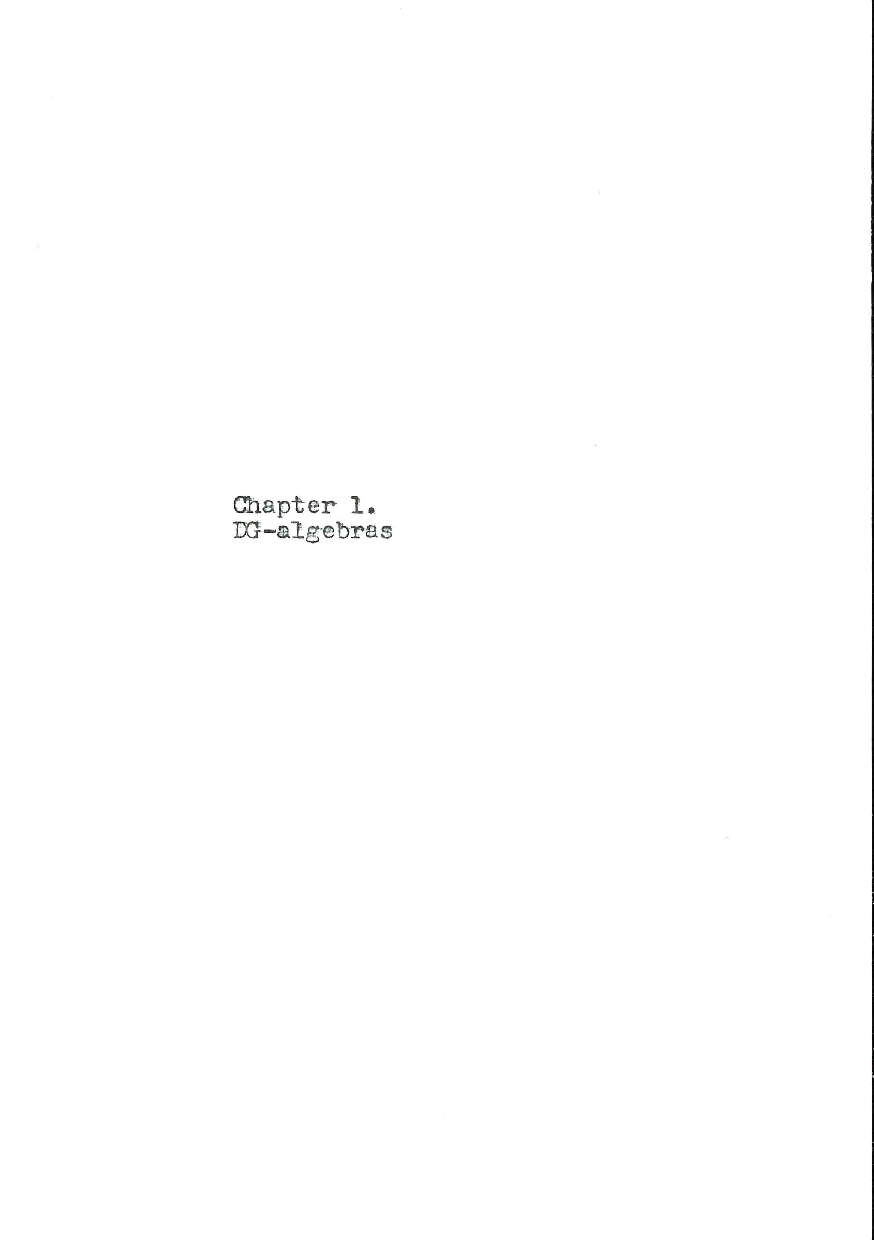
\includegraphics[%
clip,
width=1.05\paperwidth,
height=1.05\paperheight
]{chaptertitles/ch1.pdf}};

\clearpage


\subsection*{Description}

The main result of the third paper concerns a connection between three different related mathematical worlds, called the stable, the prestable and the abelian world. These three worlds are all connected by a mathematical concept called a $t$-structure. One could think of this setup as follows: in the stable world we have an infinite list of things, labeled by every positive and negative whole number. In the prestable world we only have things labeled by positive numbers, which still gives us infinitely many things, but only in one direction. In the abelian world we have only the part labeled by $0$ --- the only part right between the positive and the negative. The $t$-structure allows us to remove all of the information in any degree. For example, it can first remove all negative numbers, and then all positive numbers, leaving us only with $0$. This is precisely how it connects the stable, the prestable and the abelian worlds. I have tried to signify this passing in the drawing, where one the left we have free flowing information in all directions, while in the middle half of it is restricted in one direction. In the final rightmost part, information is restricted in both directions, leaving us only with straight lines --- no geometry, no topology. 

The colors again have no mathematical meaning, and are there only to add visual interst, and to connect to the colors of the papers. 

\newpage